\chapter{Luyện tập: Tự cảm}
\begin{enumerate}
	\item
	{
		Ống dây điện hình trụ có chiều dài tăng gấp đôi (các đại lượng khác không thay đổi) thì độ tự cảm
		\begin{mcq}(2)
			\item{không đổi.}
			\item{tăng 4 lần.}
			\item{tăng 2 lần.}
			\item{giảm 2 lần.}
		\end{mcq}
	}
	\item
	{
		Ống dây điện hình trụ có số vòng dây tăng 2 lần (các đại lượng khác không thay đổi) thì độ tự cảm
		\begin{mcq}(2)
		\item{tăng 2 lần.}
		\item{tăng 4 lần.}
		\item{giảm 2 lần.}
		\item{giảm 4 lần.}
		\end{mcq}
	}
	\item
	{
		Ống dây điện hình trụ có số vòng dây tăng 4 lần và chiều dài tăng 2 lần (các đại lượng khác không thay đổi) thì độ tự cảm
		\begin{mcq}(2)
		\item{tăng 8 lần.}
		\item{tăng 4 lần.}
		\item{giảm 2 lần.}
		\item{giảm 4 lần.}
		\end{mcq}
	}
	\item
	{
		Tính độ tự cảm của một ống dây hình trụ có chiều dài $\SI{0.5}{\meter}$ gồm $1000$ vòng dây, mỗi vòng dây có đường kính $\SI{20}{\centi \meter}$.
		\begin{mcq}(4)
		\item{$\SI{0.088}{\henry}$.}
		\item{$\SI{0.079}{\henry}$.}
		\item{$\SI{0.125}{\henry}$.}
		\item{$\SI{0.064}{\henry}$.}
		\end{mcq}	
	}
	\item
	{
		[Đề chính thức của BGD-ĐT-2018] Một cuộn cảm có độ tự cảm $\SI{0.2}{\henry}$. Trong khoảng thời gian $\SI{0.05}{\second}$, dòng điện trong cuộn cảm có cường độ giảm đều từ $\SI{2}{\ampere}$ xuống $0$ thì suất điện động tự cảm xuất hiện trong cuộn cảm có độ lớn là
		\begin{mcq}(4)
			\item{$\SI{4}{\volt}$.}
			\item{$\SI{0.4}{\volt}$.}
			\item{$\SI{0.02}{\volt}$.}
			\item{$\SI{8}{\volt}$.}
		\end{mcq}
	}
	\item
	{
		Một cuộn cảm có độ tự cảm $\SI{0.5}{\henry}$, trong đó dòng điện tăng đều với tốc độ $\SI{200}{\ampere / \second}$ thì suất điện động tự cảm là
		\begin{mcq}(4)
			\item{$\SI{-100}{\volt}$.}
			\item{$\SI{20}{\volt}$.}
			\item{$\SI{100}{\volt}$.}
			\item{$\SI{200}{\volt}$.}
		\end{mcq}
	}
		\item
	{
		Dòng điện qua một ống dây không có lõi sắt biến đổi theo thời gian. Trong thời gian $\SI{0.01}{\second}$ cường độ dòng điện tăng từ $i_1=\SI{1}{\ampere}$ đến $i_2=\SI{2}{\ampere}$, suất điện động tự cảm trong ống dây có độ lớn bằng $\SI{20}{\volt}$. Hệ số tự cảm của ống dây là
		\begin{mcq}(4)
			\item{$\SI{0.1}{\henry}$.}
			\item{$\SI{0.4}{\henry}$.}
			\item{$\SI{0.2}{\henry}$.}
			\item{$\SI{0.6}{\henry}$.}
		\end{mcq}
	}
		\item
	{
		Suất điện động tự cảm $\SI{0.75}{\volt}$ xuất hiện trong một cuộn cảm có $L=\SI{25}{\milli \henry}$, tại đó cường độ dòng điện giảm từ giá trị $I$ xuống $0$ trong $\SI{0.01}{\second}$. Tính $I$.
		\begin{mcq}(4)
			\item{$\SI{0.1}{\ampere}$.}
			\item{$\SI{0.4}{\ampere}$.}
			\item{$\SI{0.3}{\ampere}$.}
			\item{$\SI{0.6}{\ampere}$.}
		\end{mcq}
	}
			\item
	{
		Trong một mạch kín có độ tự cảm $\SI{0.5e-3}{\henry}$, nếu suất điện động tự cảm có độ lớn bằng $\SI{0.25}{\volt}$ thì tốc độ biến thiên của dòng điện là
		\begin{mcq}(4)
			\item{$\SI{250}{\ampere / \second}$.}
			\item{$\SI{400}{\ampere / \second}$.}
			\item{$\SI{600}{\ampere / \second}$.}
			\item{$\SI{500}{\ampere / \second}$.}
		\end{mcq}
	}
			\item
	{
		Một ống dây dài $l=\SI{30}{\centi \meter}$ gồm $N=1000$ vòng dây, đường kính mỗi vòng dây $d=\SI{8}{\centi \meter}$ có dòng điện với cường độ $i=\SI{2}{\ampere}$ đi qua. Tính từ thông qua mỗi vòng dây
		\begin{mcq}(4)
			\item{$\SI{42}{\micro \weber}$.}
			\item{$\SI{0.4}{\micro \weber}$.}
			\item{$\SI{0.2}{\micro \weber}$.}
			\item{$\SI{86}{\micro \weber}$.}
		\end{mcq}
	}
			\item
	{
		Một ống dây dài $l=\SI{30}{\centi \meter}$ gồm $N=1000$ vòng dây, đường kính mỗi vòng dây $d=\SI{8}{\centi \meter}$ có dòng điện với cường độ $i=\SI{2}{\ampere}$ đi qua. Thời gian ngắt dòng điện là $t=\SI{0.1}{\second}$, độ lớn suất điện động tự cảm xuất hiện trong ống dây là
		\begin{mcq}(4)
			\item{$\SI{0.15}{\volt}$.}
			\item{$\SI{0.42}{\volt}$.}
			\item{$\SI{0.24}{\volt}$.}
			\item{$\SI{8.6}{\volt}$.}
		\end{mcq}
	}
			\item
	{
		Cho mạch điện như hình vẽ.
		\begin{center}
			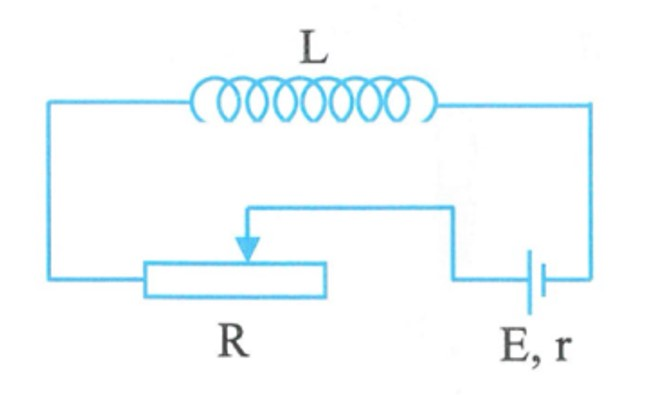
\includegraphics[scale=0.35]{../figs/VN11-PH-31-P-0211-1.jpg}
		\end{center}
	$L=\SI{1}{\henry}$, $E=\SI{12}{\volt}$, $r=0$, điện trở của biến trở là $R=\SI{10}{\Omega}$. Điều chỉnh biến trở để trong $\SI{0.1}{\second}$ điện trở của biến trở giảm còn $\SI{5}{\Omega}$.
	\begin{description}
		\item[a)] Tính suất điện động tự cảm trong ống dây trong khoảng thời gian nói trên.
		\begin{mcq}(4)
			\item{$\SI{1.2}{\volt}$.}
			\item{$\SI{2.4}{\volt}$.}
			\item{$\SI{12}{\volt}$.}
			\item{$\SI{24}{\volt}$.}
		\end{mcq}
		\item[b)] Tính cường độ dòng điện trong mạch trong khoảng thời gian nói trên.
		\begin{mcq}(4)
			\item{$\SI{0}{\ampere}$.}
			\item{$\SI{1}{\ampere}$.}
			\item{$\SI{2}{\ampere}$.}
			\item{$\SI{3}{\ampere}$.}
		\end{mcq}
		\end{description}
	}
\end{enumerate}
\hides{\textbf{Đáp án}
\begin{center}
	\begin{tabular}{|m{2.8em}|m{2.8em}|m{2.8em}|m{2.8em}|m{2.8em}|m{2.8em}|m{2.8em}|m{2.8em}|m{2.8em}|m{2.8em}|}
		\hline
		1. D & 2. B & 3. A & 4. B & 5. D & 6. A & 7. C & 8. C & 9. D & 10. A \\
		\hline
		11. B & 12a. C & 12b. A &&&&&&&\\
		\hline
	\end{tabular}
\end{center}}